% TODO: 全体的に式番号を追加する
\documentclass[a4paper,11pt]{article}
\usepackage[top=10mm]{geometry}
\usepackage{mathtools}
\usepackage{tikz}
\usetikzlibrary{calc,arrows.meta}

% --- 日本語対応（LuaLaTeX） ---
\usepackage{luatexja}
\usepackage{luatexja-fontspec}
\setmainjfont{HaranoAjiMincho}
\setsansjfont{HaranoAjiGothic}

\title{反変ベクトル、共変ベクトルとは}

\begin{document}
\maketitle

ベクトルは色々な場面で登場するが、相対論やテンソルなどちょっと進んだ内容を勉強していると、何やら$A^i, A_i$のように添字の上げ下げが現れ、反変ベクトル、共変ベクトルなどと呼ばれるようになる。
それまで単に「ベクトル」として扱っていたものが、いつの間にか2種類になってしまってよく分からないと思う人は少なくないはず。
ここでは、このような疑問を解消することを目的として、反変ベクトルと共変ベクトルについて見ていく。

\subsection*{$\bullet$ ベクトルの反変成分、共変成分}

実はベクトルの成分の取り方は二つあって、それぞれを反変成分、共変成分と呼ぶ。\\
ベクトルを基底で展開したときの

\[
  \mathbf{V} = V^i \mathbf{e}_i
\]

\noindent
この \(V^i\) が \textbf{反変成分}。(ただしここでは\textbf{Einstein規約}\footnote{
  (上下)ペアの添字について、$\Sigma$を省略して和を取る記法をEinstein規約という。このpdf内では全体的にこの記法を用いる。
}
を用いている。)\\
\noindent
一方、基底との内積をとって

\[
  V_i \coloneqq \mathbf{e}_i \cdot \mathbf{V}
\]

\noindent
としたものが \textbf{共変成分}。\\
また、ベクトルの反変成分と共変成分のことを\textbf{反変ベクトル}、\textbf{共変ベクトル}とも呼ぶ。

\subsection*{$\bullet$ 図形的意味}

上記の内容を図で表すと以下のようになる。

\medskip
\noindent
\begin{minipage}[t]{0.42\linewidth}
  \raggedright
  \underline{反変成分}\par\smallskip
  \centering
  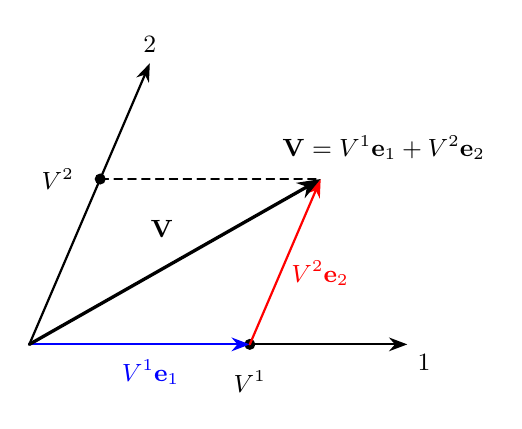
\begin{tikzpicture}[>=Stealth, line cap=round, line join=round, font=\small]

  % ===== パラメータ =====
  \coordinate (e1) at (1.0,0.0);
  \coordinate (e2) at (0.45,1.05);
  \def\Vone{2.8}
  \def\Vtwo{2.0}

  % ===== 見た目パラメータ =====
  \def\componecol{blue}   % V^1 e_1
  \def\comptwocol{red}    % V^2 e_2

  % ===== 軸 =====
  \draw[->, thick]
  (0,0) -- ($(0,0)+4.8*(e1)$) node[below right] {$1$};

  \draw[->, thick]
  (0,0) -- ($(0,0)+3.4*(e2)$) node[above] {$2$};

  % ===== 成分点 =====
  \coordinate (V1) at ($\Vone*(e1)$);
  \coordinate (V2axis) at ($\Vtwo*(e2)$);
  \coordinate (V) at ($\Vone*(e1) + \Vtwo*(e2)$);

  % ---- 1軸上の V^1 ----
  \fill (V1) circle (2pt);
  \node[below=6pt] at (V1) {$V^{1}$};

  % ---- 2軸上の V^2 ----
  \fill (V2axis) circle (2pt);
  \node[left=6pt] at (V2axis) {$V^{2}$};

  % ---- V^1 e_1（青）----
  \draw[->, thick, \componecol]
  (0,0) -- (V1)
  node[pos=0.55, below=2pt] {$V^{1}\mathbf e_{1}$};

  % ---- V^2 e_2（赤）----
  \draw[->, thick, \comptwocol]
  (V1) -- (V)
  node[pos=0.6, right=10pt, below=2pt] {$V^{2}\mathbf e_{2}$};

  % ---- V（黒・太い）----
  \draw[->, very thick]
  (0,0) -- (V)
  node[pos=0.55, above left=2pt] {$\mathbf V$};

  % ---- 補助線 ----
  \draw[densely dashed] (0,0) -- (V2axis);
  \draw[densely dashed] (V2axis) -- (V);

  % ---- 式 ----
  \node at (4.5,2.5)
  {$\mathbf V = V^{1}\mathbf e_{1} + V^{2}\mathbf e_{2}$};

\end{tikzpicture}

\end{minipage}
\hspace{0.10\linewidth}
\begin{minipage}[t]{0.42\linewidth}
  \raggedright
  \underline{共変成分}\par\smallskip
  \centering
  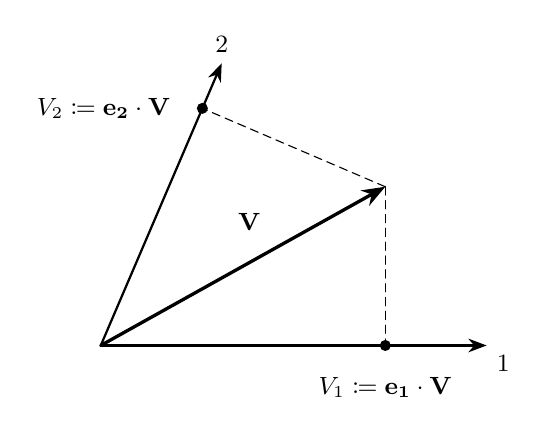
\begin{tikzpicture}[>=Stealth, line cap=round, line join=round, font=\small]

  % ===== パラメータ =====
  \coordinate (O) at (0,0);
  \coordinate (e1) at (1.0,0.0);
  \coordinate (e2) at (0.48,1.12);
  \def\Vone{2.75}
  \def\Vtwo{1.8}

  % ===== 軸 =====
  \draw[->, thick]
  (O) -- ($(O)+4.9*(e1)$) node[below right] {$1$};

  \draw[->, thick]
  (O) -- ($(O)+3.2*(e2)$) node[above] {$2$};

  % ===== 点 =====
  \coordinate (V) at ($(O)+\Vone*(e1)+\Vtwo*(e2)$);
  \coordinate (e1ref) at ($(O)+(e1)$);
  \coordinate (e2ref) at ($(O)+(e2)$);
  \coordinate (VoneAxis) at ($(O)!(V)!(e1ref)$);
  \coordinate (VtwoAxis) at ($(O)!(V)!(e2ref)$);

  % ===== ベクトル V =====
  \draw[->, very thick]
  (O) -- (V)
  node[pos=0.62, above left=2pt] {$\mathbf V$};

  % ===== 共変成分への射影 =====
  \draw[densely dashed] (V) -- (VoneAxis);
  \draw[densely dashed] (V) -- (VtwoAxis);
  % TODO: 垂直記号が上手くいかない
  % \draw ($(VoneAxis)!0.16!(V)$) -- ++(0,0.16) -- ++(0.16,0);
  % \draw ($(VtwoAxis)!0.16!(V)$) -- ($($(VtwoAxis)!0.16!(V)$)+(0.14,0.06)$) -- ($($(VtwoAxis)!0.16!(V)$)+(0.08,0.20)$);

  % ===== 軸上の成分点 =====
  \fill (VoneAxis) circle (2pt);
  \node[below=8pt] at (VoneAxis) {$V_{1}\coloneq\mathbf{e_{1}}\cdot\mathbf{V}$};

  \fill (VtwoAxis) circle (2pt);
  \node[left=8pt] at (VtwoAxis) {$V_{2}\coloneq\mathbf{e_{2}}\cdot\mathbf{V}$};

\end{tikzpicture}

\end{minipage}

\newpage

\subsection*{$\bullet$ 計量を使った表現}

共変成分は

\[
  V_i = \mathbf{e}_i \cdot \mathbf{V}
  = \mathbf{e}_i \cdot (V^j \mathbf{e}_j)
  = (\mathbf{e}_i \cdot \mathbf{e}_j)V^j
\]

\noindent
となるので、

\[
  g_{ij} \coloneqq \mathbf{e}_i \cdot \mathbf{e}_j
\]

\noindent
とすると

\[
  V_i = g_{ij}V^j
\]

\noindent
と表せる。$g_{ij}$を計量テンソルと呼ぶ。

\subsection*{$\bullet$ デカルト座標では反変成分と共変成分が一致する}

\textbf{デカルト座標では}、計量が

\[
  g_{ij} = \delta_{ij}
\]

\noindent
だから

\[
  V_i = \delta_{ij}V^j = V^i
\]

\noindent
となって、\textbf{反変成分と共変成分が一致する}。


\subsection*{$\bullet$ 反変、共変の由来}

反変、共変の由来は基底変換時の挙動にある。\\
そこで、

\[
  \mathbf{e}_{i'} = a_{i'}{}^j \mathbf{e}_j
\]

\noindent
このような基底変換に対して、$V^i$と$V_i$がどのように変換されるかを考える。\\
まず、反変成分に関しては、

\begin{align*}
  \mathbf{V} & = V^i \mathbf{e}_i                 \\
             & = V^{i'} \mathbf{e}_{i'}           \\
             & = V^{i'} (a_{i'}{}^j \mathbf{e}_j) \\
             & = (a_{i'}{}^j V^{i'}) \mathbf{e}_j \\
             & = (a_{j'}{}^i V^{j'}) \mathbf{e}_i
\end{align*}

\noindent
最初と最後を比較して、

\[
  V^i = a_{j'}{}^i V^{j'}
\]

\noindent
よって、

\[
  V^{i'} = (a^{-1})_{j}{}^{i'} V^{j}
\]

\noindent
となる。つまり、\textbf{反変成分は基底変換に対してその逆変換を受ける}。\\
一方、共変成分は、

\begin{align*}
  V_{i'} & = g_{i'j'}V^{j'}                                                                       \\
         & = (\mathbf{e}_{i'}\cdot \mathbf{e}_{j'})V^{j'}                                         \\
         & = a_{i'}{}^{l} a_{j'}{}^{m} (\mathbf{e}_l \cdot \mathbf{e}_m)(a^{-1})_{n}{}^{j'} V^{n} \\
         & = a_{i'}{}^{l} (a^{-1})_{n}{}^{j'} a_{j'}{}^m g_{lm} V^{n}                             \\
         & = a_{i'}{}^{l} \delta^m_n g_{lm}V^n                                                    \\
         & = a_{i'}{}^l g_{ln}V^n                                                                 \\
         & = a_{i'}{}^{l} V_l
\end{align*}

\noindent
となる。つまり、\textbf{共変成分は基底変換と同様に変換される}。\\

\noindent
※ここでは基底を使って反変、共変を定義したけど、物理だとこの変換性から定義することが多い。

\end{document}
